% SPDX-License-Identifier: LicenseRef-DPS8M-Doc AND LicenseRef-CFGAL
% SPDX-FileCopyrightText: 2019-2021 Dean S. Anderson
% SPDX-FileCopyrightText: 2021-2022 The DPS8M Development Team

\section[Simulator Configuration / Operation]{SIMULATOR CONFIGURATION / OPERATION}

This section covers the configuration of the simulator and how to change it.

Note that the default configuration contains more hardware in it than Multics can handle (see the MULTICS CONFIGURATION section warning).
So you want to pick and choose which parts of the configuration meet your needs. The MULTICS CONFIGURATION section shows how to do this.

First, the following diagrams show the default configuration of the simulator
when it first starts up.

\subsection[CPU/SCU Default Configuration]{CPU/SCU DEFAULT CONFIGURATION}

By default there are 6 CPUs, 4 SCUs (with max memory) and 2 IOMs. In most systems, using 2 to 4 of the CPUs will be sufficent. Since each of the
4 SCUs is configured with 16 Mw, the maximum amount of memory is available (64 Mw). That is the maximum phyiscal memory the simulator can provide (and
Multics can make use of). Here is how these devices are cabled:

\noindent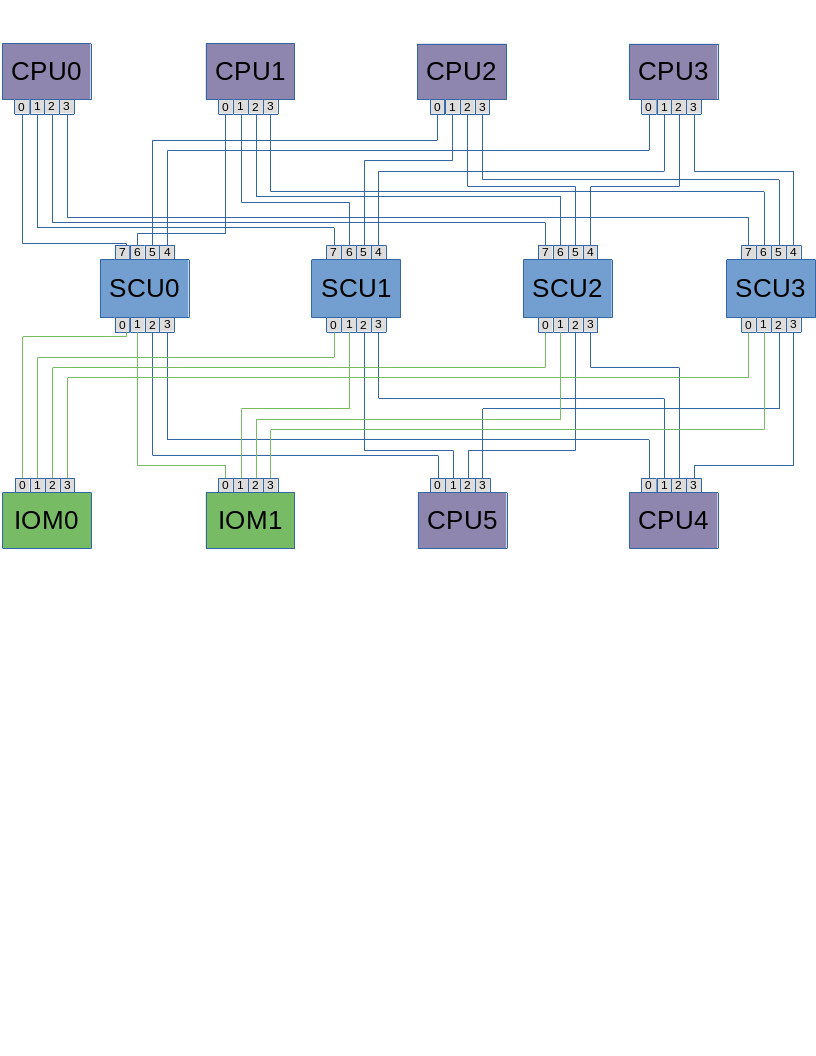
\includegraphics[width=\textwidth,height=\textheight,keepaspectratio]{DefaultCablingDiagram-cpu.png}

\subsection[IOM0 Default Configuration]{IOM0 DEFAULT CONFIGURATION}

\noindent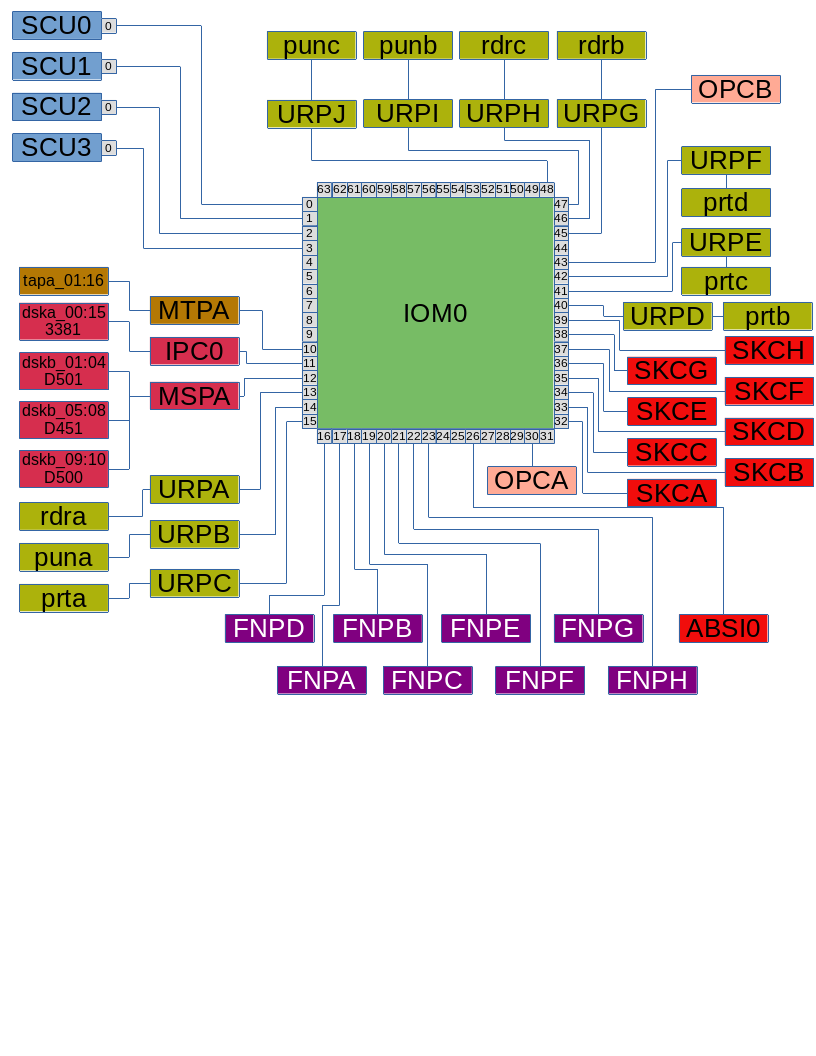
\includegraphics[width=\textwidth,height=\textheight,keepaspectratio]{DefaultCablingDiagram-IOM0.png}

\subsection[IOM1 Default Configuration]{IOM1 DEFAULT CONFIGURATION}

\noindent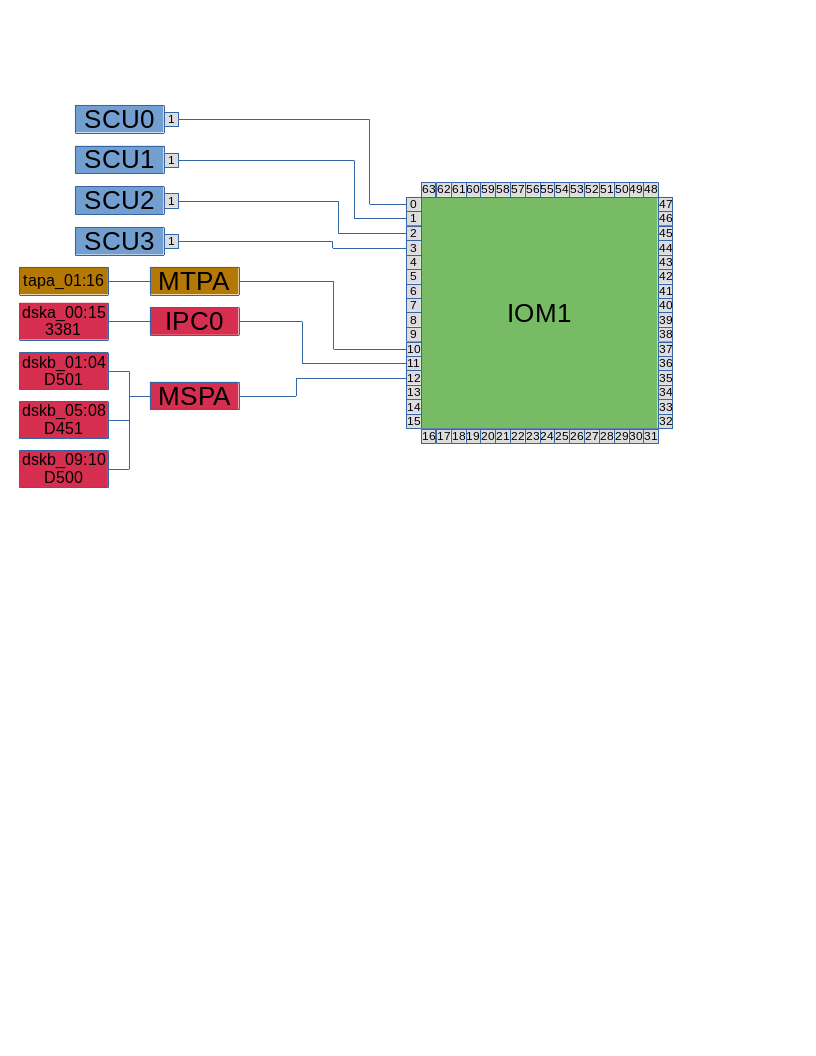
\includegraphics[width=\textwidth,height=\textheight,keepaspectratio]{DefaultCablingDiagram-IOM1.png}
